
\documentclass[a4paper,11pt]{article}
\usepackage[a4paper, margin=8em]{geometry}

% usa i pacchetti per la scrittura in italiano
\usepackage[french,italian]{babel}
\usepackage[T1]{fontenc}
\usepackage[utf8]{inputenc}
\frenchspacing 

% usa i pacchetti per la formattazione matematica
\usepackage{amsmath, amssymb, amsthm, amsfonts}

% usa altri pacchetti
\usepackage{gensymb}
\usepackage{hyperref}
\usepackage{standalone}

% imposta il titolo
\title{Appunti Elettronica Digitale}
\author{Luca Seggiani}
\date{2026}

% imposta lo stile
% usa helvetica
\usepackage[scaled]{helvet}
% usa palatino
\usepackage{palatino}
% usa un font monospazio guardabile
\usepackage{lmodern}

\renewcommand{\rmdefault}{ppl}
\renewcommand{\sfdefault}{phv}
\renewcommand{\ttdefault}{lmtt}

% disponi il titolo
\makeatletter
\renewcommand{\maketitle} {
	\begin{center} 
		\begin{minipage}[t]{.8\textwidth}
			\textsf{\huge\bfseries \@title} 
		\end{minipage}%
		\begin{minipage}[t]{.2\textwidth}
			\raggedleft \vspace{-1.65em}
			\textsf{\small \@author} \vfill
			\textsf{\small \@date}
		\end{minipage}
		\par
	\end{center}

	\thispagestyle{empty}
	\pagestyle{fancy}
}
\makeatother

% disponi teoremi
\usepackage{tcolorbox}
\newtcolorbox[auto counter, number within=section]{theorem}[2][]{%
	colback=blue!10, 
	colframe=blue!40!black, 
	sharp corners=northwest,
	fonttitle=\sffamily\bfseries, 
	title=~\thetcbcounter: #2, 
	#1
}

% disponi definizioni
\newtcolorbox[auto counter, number within=section]{definition}[2][]{%
	colback=red!10,
	colframe=red!40!black,
	sharp corners=northwest,
	fonttitle=\sffamily\bfseries,
	title=~\thetcbcounter: #2,
	#1
}

% U.D.M
\newcommand{\amp}{\ensuremath{\mathrm{A}}}
\newcommand{\volt}{\ensuremath{\mathrm{V}}}
\newcommand{\meter}{\ensuremath{\mathrm{m}}}
\newcommand{\second}{\ensuremath{\mathrm{s}}}
\newcommand{\farad}{\ensuremath{\mathrm{F}}}
\newcommand{\henry}{\ensuremath{\mathrm{H}}}
\newcommand{\siemens}{\ensuremath{\mathrm{S}}}

% circuiti
\usepackage{circuitikz}
\usetikzlibrary{babel}

% disegni
\usepackage{pgfplots}
\pgfplotsset{width=10cm,compat=1.9}

% disponi codice
\usepackage{listings}
\usepackage[table]{xcolor}

\definecolor{codegreen}{rgb}{0,0.6,0}
\definecolor{codegray}{rgb}{0.5,0.5,0.5}
\definecolor{codepurple}{rgb}{0.58,0,0.82}
\definecolor{backcolour}{rgb}{0.95,0.95,0.92}

\lstdefinestyle{codestyle}{
		backgroundcolor=\color{black!5}, 
		commentstyle=\color{codegreen},
		keywordstyle=\bfseries\color{magenta},
		numberstyle=\sffamily\tiny\color{black!60},
		stringstyle=\color{green!50!black},
		basicstyle=\ttfamily\footnotesize,
		breakatwhitespace=false,         
		breaklines=true,                 
		captionpos=b,                    
		keepspaces=true,                 
		numbers=left,                    
		numbersep=5pt,                  
		showspaces=false,                
		showstringspaces=false,
		showtabs=false,                  
		tabsize=2
}

\lstdefinestyle{shellstyle}{
		backgroundcolor=\color{black!5}, 
		basicstyle=\ttfamily\footnotesize\color{black}, 
		commentstyle=\color{black}, 
		keywordstyle=\color{black},
		numberstyle=\color{black!5},
		stringstyle=\color{black}, 
		showspaces=false,
		showstringspaces=false, 
		showtabs=false, 
		tabsize=2, 
		numbers=none, 
		breaklines=true
}

\lstdefinelanguage{javascript}{
	keywords={typeof, new, true, false, catch, function, return, null, catch, switch, var, if, in, while, do, else, case, break},
	keywordstyle=\color{blue}\bfseries,
	ndkeywords={class, export, boolean, throw, implements, import, this},
	ndkeywordstyle=\color{darkgray}\bfseries,
	identifierstyle=\color{black},
	sensitive=false,
	comment=[l]{//},
	morecomment=[s]{/*}{*/},
	commentstyle=\color{purple}\ttfamily,
	stringstyle=\color{red}\ttfamily,
	morestring=[b]',
	morestring=[b]"
}

% disponi sezioni
\usepackage{titlesec}

\titleformat{\section}
	{\sffamily\Large\bfseries} 
	{\thesection}{1em}{} 
\titleformat{\subsection}
	{\sffamily\large\bfseries}   
	{\thesubsection}{1em}{} 
\titleformat{\subsubsection}
	{\sffamily\normalsize\bfseries} 
	{\thesubsubsection}{1em}{}

% disponi alberi
\usepackage{forest}

\forestset{
	rectstyle/.style={
		for tree={rectangle,draw,font=\large\sffamily}
	},
	roundstyle/.style={
		for tree={circle,draw,font=\large}
	}
}

% disponi algoritmi
\usepackage{algorithm}
\usepackage{algorithmic}
\makeatletter
\renewcommand{\ALG@name}{Algoritmo}
\makeatother

% disponi numeri di pagina
\usepackage{fancyhdr}
\fancyhf{} 
\fancyfoot[L]{\sffamily{\thepage}}

\makeatletter
\fancyhead[L]{\raisebox{1ex}[0pt][0pt]{\sffamily{\@title \ \@date}}} 
\fancyhead[R]{\raisebox{1ex}[0pt][0pt]{\sffamily{\@author}}}
\makeatother

\begin{document}
% sezione (data)
\section{Lezione del 30-03-26}

% stili pagina
\thispagestyle{empty}
\pagestyle{fancy}

% testo
\subsection{Modello del BJT ai piccoli segnali}
Iniziamo a vedere come studiare un modello del BJT adatto all'analisi dei \textit{piccoli segnali}.

Anche qui adotteremo un approccio simile a quello visto in 9.1, cioè dove linearizziamo attorno ad un punto di equilibrio. Iniziamo dalle caratteristiche di ingresso e di uscita ormai ampiamente viste:
$$
\begin{cases}
	V_{BE} = f(I_B, V_{CE}) \\
	I_C = g(I_B, V_{CE})
\end{cases}
$$
e prevediamo un punto di linearizzazione $Q$ (o di \textit{quiescenza}) dei parametri $I_B$ e $V_{CE}$:
$$
\begin{cases}
	I_B(t) = I_{BQ} + i_b (t) \\
	V_{CE}(t) = V_{CEQ} + v_{ce}(t)
\end{cases}
$$
per cui le caratteristiche di ingresso e uscita diventeranno:
$$
\begin{cases}
	V_{BE} = f(I_{BQ} + i_b(t), V_{CEQ} + v_{ce}(t)) \\
	I_C = g(I_{BQ} + i_b(t), V_{CEQ} + v_{ce}(t))
\end{cases}
$$

Procediamo quindi ad esprimere, sempre come avevamo fatto in 9.1, la decomposizione di Taylor troncata al termine linare di etnrambe le caratteristiche:
$$
\begin{cases}
	V_{BE} = f(I_{BQ}) + \frac{\partial f}{\partial i_B} \Big|_{I_{BQ}, V_{CEQ}} \cdot i_b(t) + \frac{\partial f}{\partial v_{ce}} \Big|_{I_{BQ}, V_{CEQ}} \cdot v_{ce}(t) = V_{BEQ} + v_{be}(t) \\

	I_C = g(I_{BQ}) + \frac{\partial g}{\partial i_B} \Big|_{I_{BQ}, V_{CEQ}} \cdot i_b(t) + \frac{\partial g}{\partial v_{ce}} \Big|_{I_{BQ}, V_{CEQ}} \cdot v_{ce}(t) = I_{CQ} + i_c(t) \\
\end{cases}
$$
dove i termini linearizzati sono::
$$
\begin{cases}
v_{be}(t) \approx \frac{\partial f}{\partial I_B} \Big|_Q \cdot i_b(t) + \frac{\partial f}{\partial V_{CE}} \Big|_Q \cdot v_{ce}(t) \\

i_c(t) \approx \frac{\partial g}{\partial I_B} \Big|_Q \cdot i_b(t) + \frac{\partial g}{\partial V_{CE}} \Big|_Q \cdot v_{ce}(t) \\
\end{cases}
$$

\par\smallskip

\newpage

\noindent
\textbf{\textsf{Parametri ibridi}}

\noindent
I parametri differenziali in forma:
$$
\frac{\partial \{ f, \, g \} }{\partial \{ I_B \, V_{CE} \} } \Big|_Q
$$
si prestano ad una parametrizzazione a \textbf{parametri ibridi}, già vista ad esempio nei testi di elettrotecnica.
In particolare possiamo definire i parametri:
$$
\begin{cases}
h_{ie} = \overline{h_{11}} = \frac{\partial f}{\partial I_B} \Big|_Q \\
h_{re} = \overline{h_{12}} = \frac{\partial f}{\partial V_{CE}} \Big|_Q \\ 
h_{fe} = \overline{h_{21}} = \frac{\partial g}{\partial I_B} \Big|_Q \\
h_{oe} = \overline{h_{22}} = \frac{\partial g}{\partial V_{CE}} \Big|_Q
\end{cases}
$$

Ricordiamo dai testi che la forma generale di una sintesi a parametri h è:
\[
	\begin{cases}
		\dot{V}_1 = \overline{h_{11}} \dot{I}_1 + \overline{h_{12}} \dot{V}_2 \\ 
		\dot{I}_2 = \overline{h_{21}} \dot{I}_1 + \overline{h_{22}} \dot{V}_2
	\end{cases}
\]
o come matrice:
$$
\begin{pmatrix}
	\dot{V}_1 \\ \dot{I}_2
\end{pmatrix}
= \overline{h}
\begin{pmatrix}
	\dot{I}_1 \\ \dot{V}_2
\end{pmatrix}
$$

Su un transistor prendiamo la corrente $i_1$ come la $I_B$ entrante alla base,, la $i_2$ come la $I_C$ entrante al collettore, e chiaramente l'emettitore comune. Questo è meglio esemplificato dal seguente schema:
\begin{center}
	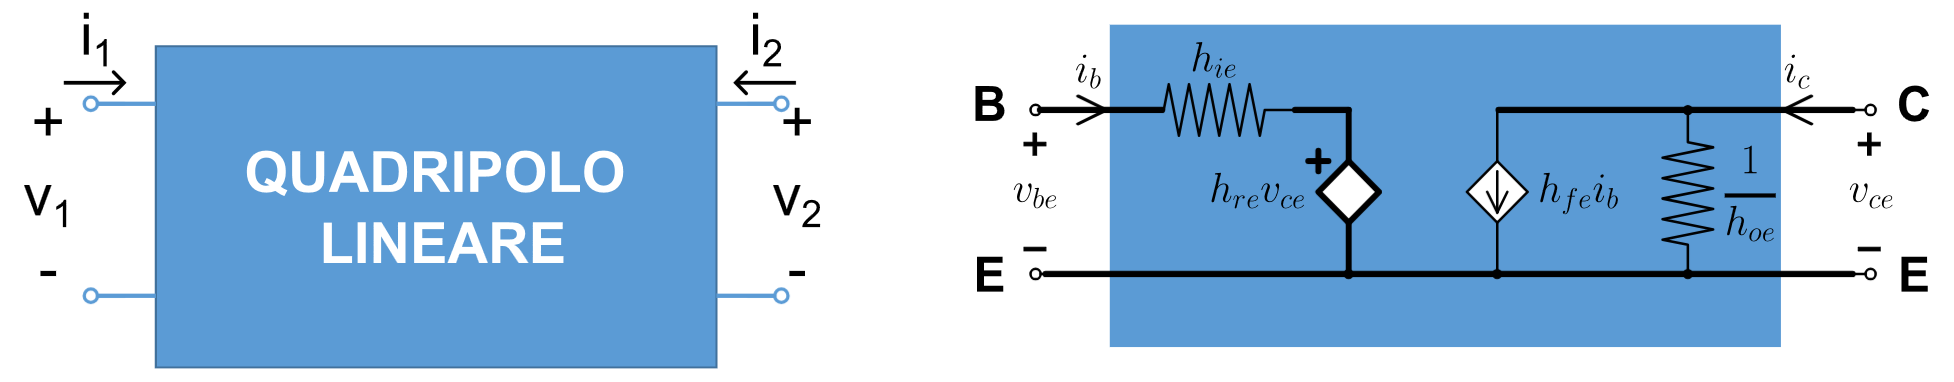
\includegraphics[scale=0.2]{../figures/bjt_hybrid.png}
\end{center}



Le componenti di $\overline{h}$ si ricavano quindi come:
$$
h:
\begin{pmatrix}
	h_{ie} = \overline{h_{11}} = \frac{\dot{V}_1}{\dot{I}_1} \Big|_{\dot{V}_2 = 0} &
	h_{re} = \overline{h_{12}} = \frac{\dot{V}_1}{\dot{V}_2} \Big|_{\dot{I}_1 = 0} \\
	h_{fe} = \overline{h_{21}} = \frac{\dot{I}_2}{\dot{I}_1} \Big|_{\dot{V}_2 = 0} &
	h_{oe} = \overline{h_{22}} = \frac{\dot{I}_2}{\dot{V}_2} \Big|_{\dot{I}_1 = 0}
\end{pmatrix}
$$

Questo tipo di sintesi ha un significato interessante sui vari parametri, e in particolare su dispositivi come il BJT, in quanto associa ogni parametro ad una particolare proprietà del transistor:
\begin{itemize}
	\item $\overline{h_{11}}$: impedenza di ingresso;
	\item $\overline{h_{12}}$: guadagno di tensione inverso;
	\item $\overline{h_{21}}$: guadagno di corrente diretto;
	\item $\overline{h_{22}}$: ammettenza di uscita.
\end{itemize}

\par\smallskip

\noindent
\textbf{\textsf{Circuito equivalente}}

\noindent
Il circuito equivalente che possiamo formare da una rappresentazione a parametri ibridi è il seguente: 
\begin{center}
	\begin{circuitikz}
		\draw (-4, 1) -- (-3, 1) 
			to [ european resistor, l=$\overline{h_{11}}$, i=$I_1$] (-1, 1)
			to [ controlled voltage source, v<=$\overline{h_{12}} \dot{V}_2$ ] (-1, -1) 
			to [ short, i=$I_1$ ] (-3, -1)	
			-- (-4, -1);
			
		\draw (-4.6, 1) node[anchor=west] {$+$};
		\draw (-4.6, 0) node[anchor=west] {$V_1$};
		\draw (-4.6, -1) node[anchor=west] {$-$};

		\draw (6,1) to [ short, i=$I_2$] (5, 1) 
			to [ short] (3, 1)
			to [ controlled current source, cI_>=$\overline{h_{21}} \dot{I}_2$ ] (3, -1) 
			to [ short] (5, -1)
			-- (6, -1);
	
		\draw (6.6, 1) node[anchor=east] {$+$};
		\draw (6.6, 0) node[anchor=east] {$V_2$};
		\draw (6.6, -1) node[anchor=east] {$-$};
		
		\draw (4, 1) to [ european resistor, l=$\frac{1}{\overline{h_{22}}}$] (4, -1);

		\node[rectangle, draw, minimum width = 8.5cm, minimum height = 4cm] (a) at (1,0) {};
	\end{circuitikz}
\end{center}
da cui l'impedenza $\overline{h_{11}}$ e l'ammettenza $\overline{h_{22}}$ vengono rese come impedenze rispetivamente in serie e in parallelo, l'inverso dell'amplificazione di tensione $\overline{h_{12}}$ come il coefficiente di un generatore di tensione pilotato, e l'amplificazione di corrente $\overline{h_{21}}$ come il coefficiente di un generatore di corrente pilotato.

\par\smallskip

\noindent
\textbf{\textsf{Significato dei parametri}}

\noindent
Approfondiamo qual'è il significato dal punto di vista fisico dei parametri ibridi appena calcolati sul BJT.
\begin{itemize}
\item \textbf{\textsf{Impedenza di ingresso}} $h_{ie} = \overline{h_{11}}$ \\
Questo parametro corrisponde al rapporto fra la tensione $V_{BE}$ alla base e la corrente $I_B$ che riusciamo a far scorrere. In questo, è una misura diretta della pendenza della curva di risposta della caratteristica in ingresso:
\begin{center}
	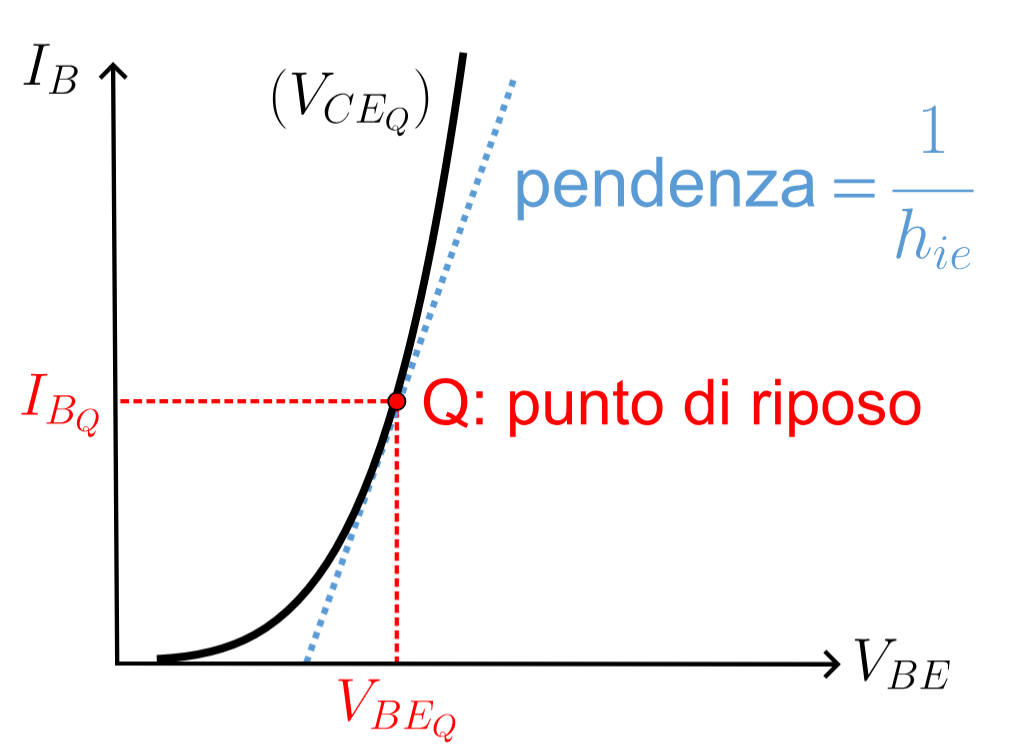
\includegraphics[scale=0.2]{../figures/trans_h_ie.png}
\end{center}
Risulta analoga alla resistenza differenziale del diodo (con la giunzione BE in ZAD).

\item \textbf{\textsf{Guadagno di tensione inverso}} $h_{re} = \overline{h_{12}}$ \\
	Questo parametro rappresenta il guadagno di tensione che abbiamo sulla porta di ingresso (la base-emettitore). In questo modellizza il risultato dell'effetto Early sulla caratteristica di ingresso, cioè la dipendenza dal voltaggio $V_{CE}$ alla porta di uscita.
\begin{center}
	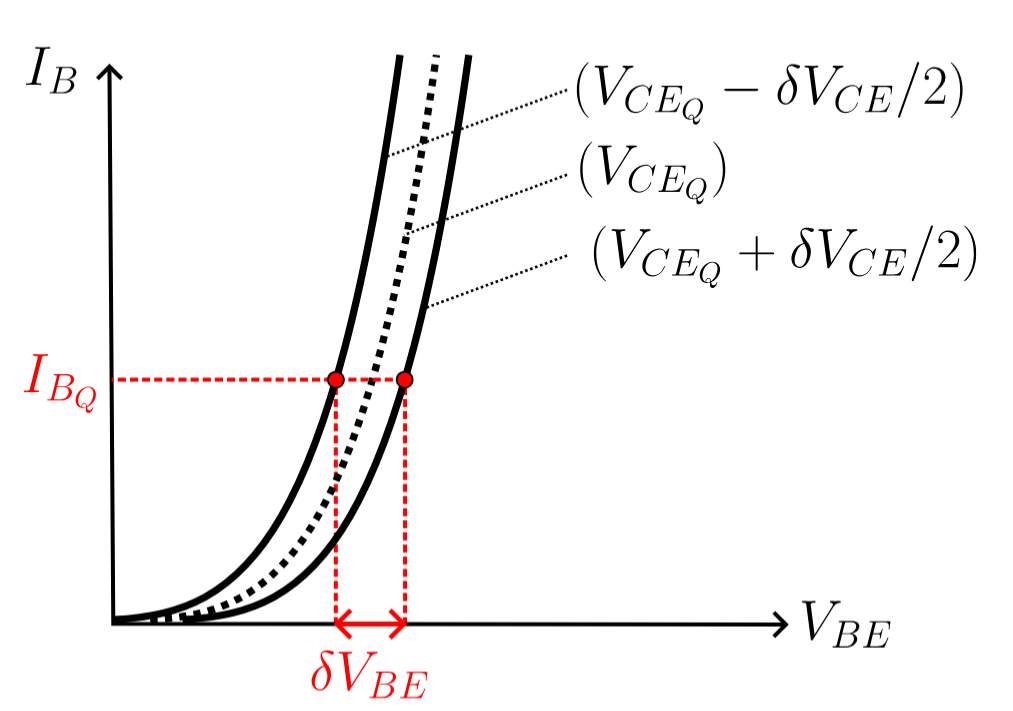
\includegraphics[scale=0.2]{../figures/trans_h_re.png}
\end{center}

\item \textbf{\textsf{Guadagno di corrente diretto}} $h_{fe} = \overline{h_{21}}$ \\
Questa è la costante che lega la corrente in entrata alla porta di ingresso (la base) alla corrente in $I_C$. In questa è direttamente legata al fattore di guadagno in corrente $\beta_F$:
$$
I_C = \beta_F I_B
$$
anche se notiamo che nel parametro $h_{fe}$ reale, ottenuto linearizzando il transistore su un punto di riposo $Q$, $h_{fe}$ è leggermente superiore a $\beta_F$.
\begin{center}
	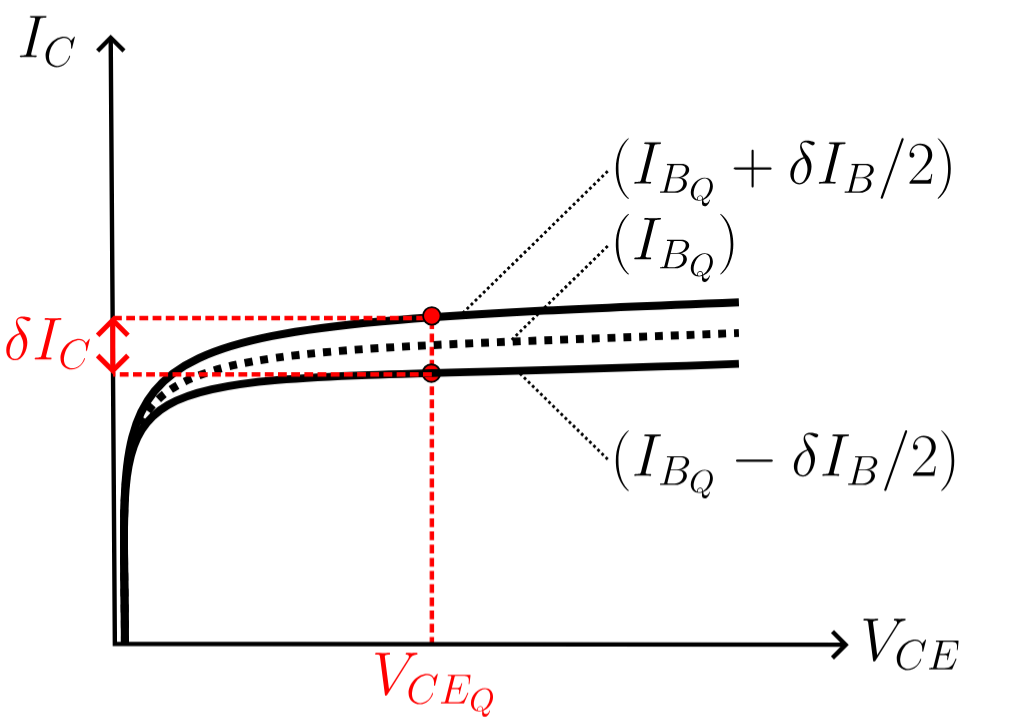
\includegraphics[scale=0.2]{../figures/trans_h_fe.png}
\end{center}

\item \textbf{\textsf{Ammettenza di uscita}} $h_{oe} = \overline{h_{22}}$ \\
Infine, questo parametro (o meglio il suo opposto) rappresenta l'impedenza sulla porta di uscita, quindi la piccola resistenza che vi associavamo per causa dell'effetto di Early. 

In termini grafici, è legato alla pendneza della curva della caratteristica di uscita nel punto di linearizzazione:
\begin{center}
	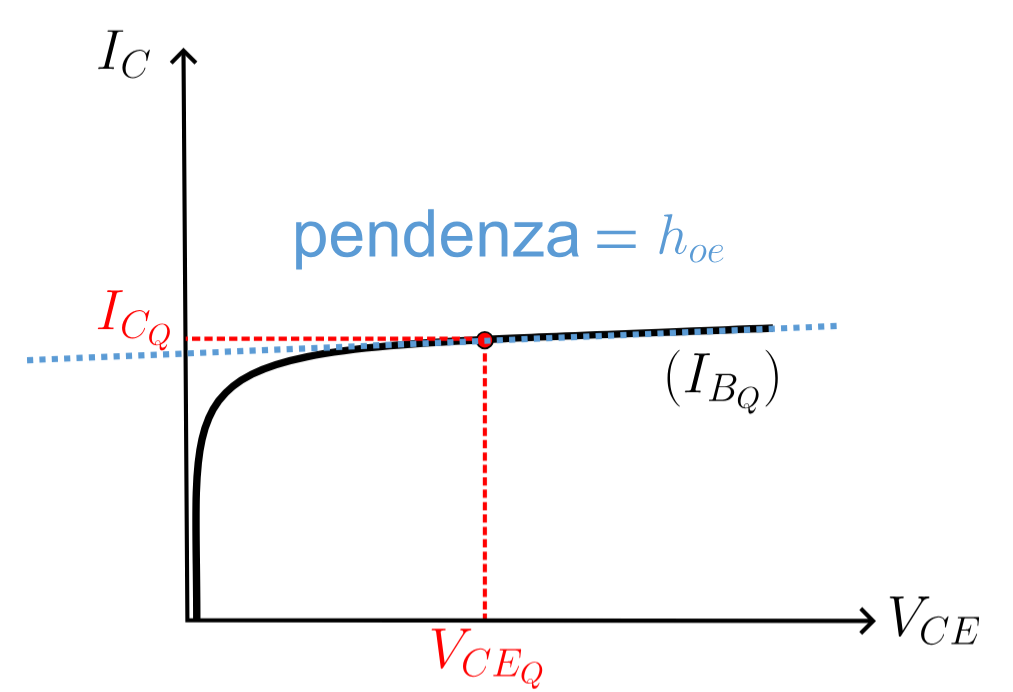
\includegraphics[scale=0.2]{../figures/trans_h_oe.png}
\end{center}

\end{itemize}

Abbiamo quindi trovato un altro modello per il transistor BJT, che possiamo affiancare ad i modelli già trovati per i BJT PNP e NPN. Notiamo che il modello è equivalente per entrambi i tipi di transistor, ovvero sia il PNP che l'NPN collassano allo stesso modello (e quindi pressappoco lo stesso comportamento) ai piccoli segnali. 

\newpage

\subsection{Accoppiamento AC}
Riprendiamo l'amplificatore a 4 resistori visto in 11.2.1, e vediamo cosa accade se si collega il segnale direttamente alla base del BJT, e il carico direttamente al collettore. Chiamiamo questo accoppiamento anche \textit{accoppiamento DC}.

\begin{center}
\begin{circuitikz}
	\draw
(0,0) node[ground]{} to[R=$R_2$] (0,3)
to[R=$R_1$] (0,6) node[vcc]{};

\draw (0,3) -- (2,3);

\draw (2,3) node[npn, anchor=B] (Q1) {};

\draw (Q1.C) to[R=$R_C$] ++(0,3) node[vcc]{};
\draw (Q1.E) to[R=$R_E$] ++(0,-3) node[ground]{};

\draw[->] (1.2,3.3) -- (1.8,3.3) node[midway, above]{$I_B$};
\draw[->] (Q1.C) ++(0.3,0.5) -- ++(0,-1) node[midway, right]{$I_C$};
\draw[->] (Q1.E) ++(0.3,0) -- ++(0,-.8) node[midway, right]{$I_E$};

\node[ground] at(-3, 0) {};
\draw (-3, 0) to [ voltage source, v=$V_s$] (-3, 3)
	to [resistor, l=$R_s$] (0, 3);

\node[ground] at(6, 0) {};
\draw(3, 4.5) -- (6, 4.5)
	to[resistor, l=$R_L$] (6, 0);

\end{circuitikz}
\end{center}

Notiamo subito che questa situazione è fallimentare. Possiamo applicare Thevenin alla rete di sinistra (quella collegata alla base del BJT) per trovare il voltaggio equivalente alla base. Inoltre, possiamo calcolare separatamente i casi con un solo generatore ($V_{cc}$ e $V_s$) attaccato, e quindi applicare la sovrapposizione degli effetti:
\begin{itemize}
	\item Per $V_s \neq 0$ e $V_{cc} = 0$ abbiamo che la coppia $R_1$, $R_2$ è collegata in parallelo a massa, e quindi la $V_{THEV}$ equivalente si calcola come:
$$
V_{THEV}' = V_s \frac{R_1 || R_2}{R_1 || R_2 + R_s}
$$
cioè la tensione data dal partitore di tensione formato dalla coppia $R_1 || R_2$ e $R_s$;

	\item Per $V_s = 0$ e $V_{cc} \neq 0$ abbiamo invece che la coppia $R_s$, $R_2$ è collegata in parallelo a massa, e quindi la $V_{THEV}$ equivalente si calcola come:
$$
V_{THEV}'' = V_{cc} \frac{R_s || R_2}{R_s || R_2 + R_1}
$$
cioè la tensione data dal partitore di tensione formato dalla coppia $R_s || R_2$ e $R_1$.

\end{itemize}

Trovata la tensione alla base, calcoliamo con lo stesso metodo la tensione sull'alimentaione del transistor (al collettore):
$$
V_{cc} \frac{R_L}{R_L + R_C}
$$
dato dal partitore di tensione formato da $R_L$ al carico e $R_C$ al collettore, che si trovano in serie.

Seguiranno quindi alcune considerazioni:
\begin{itemize}
	\item Se $R_L << R_0$, l'alimentazione $V_{cc} \frac{R_L}{R_L + R_C}$ andrà a tendere a 0, e quindi tenderà a zero anche la $V_{CEQ}$. Il transistore BJT lavorerà quindi nel regime di saturazione, dove abbiamo detto non è efficiente come amplificatore;
	\item Se $R_S << R_1, R_2$, la tensione alla base tenderà a zero ($V_s$ spento per sovrapposizione degli effetti). Se anche la base va a zero, il transistor torna a lavorare poco, e addirittura si spenge per $V_{BE} < V_\gamma$.
\end{itemize}

Abbiamo quindi che, in generale, si presenta il seguente problema: l’accoppiamento DC interferisce con la polarizzazione (il punto $Q$) del BJT.

\par\smallskip

La soluzione che daremo a questo problema sarà quello di usare il cosiddetto \textit{accoppiamento AC}:

\begin{center}
\begin{circuitikz}
	\draw
(0,0) node[ground]{} to[R=$R_2$] (0,3)
to[R=$R_1$] (0,6) node[vcc]{};

\draw (0,3) -- (2,3);

\draw (2,3) node[npn, anchor=B] (Q1) {};

\draw (Q1.C) to[R=$R_C$] ++(0,3) node[vcc]{};
\draw (Q1.E) to[R=$R_E$] ++(0,-3) node[ground]{};

\draw[->] (1.2,3.3) -- (1.8,3.3) node[midway, above]{$I_B$};
\draw[->] (Q1.C) ++(0.3,0.5) -- ++(0,-1) node[midway, right]{$I_C$};
\draw[->] (Q1.E) ++(0.3,0) -- ++(0,-.8) node[midway, right]{$I_E$};

\node[ground] at(-4, 0) {};
\draw (-4, 0) to [ voltage source, v=$V_s$] (-4,3)
	to [resistor, l=$R_s$] (-2, 3)
	to [capacitor, l=$C_s$] (0, 3);

\node[ground] at(6, 0) {};
\draw(3, 4.5) to[ capacitor, l=$C_L$] (6, 4.5)
	to[resistor, l=$R_L$] (6, 0);

\end{circuitikz}
\end{center}

In questo accoppiamento mettiamo due condensatori ($C_s$ al segnale e $C_L$ al carico), detti \textit{condensatori di disaccoppiamento}. Abbiamo quindi che come nell'accoppiamento DC sia il generatore di sorgente che il carico vengono connessi al BJT (con lo schema di polarizzazione a 4 resistori), ma stavolta tramite i condensatori di disaccoppiamento $C_s$, $C_L$.

Vediamo come questi risolvono il problema:
\begin{itemize}
	\item In corrente continua (DC), i condensatori offrono una impedenza infinita, aprendo le maglie relative alla sorgente e al carico. Il punto $Q$ del BJT viene quindi determinato unicamente dallo schema di polarizzazione a 4 resistori;
	\item In alternata (AC), i condensatori si considerano corto-circuiti, permettendo al segnale (tempo-variante) di attraversare lo stadio amplificatore e
raggiungere il carico (questo è il regime di operazione che vogliamo dall'amplificatore).
\end{itemize}

Abbiamo quindi risolto il problema. Vediamo però che le frequenze per cui i condensatori possono considerarsi in cortocircuito dipendono dalla resistenza vista da ciascuno di essi:
$$
\omega_{z,X} = \frac{1}{R_X C_X}
$$
È possibile calcolare $R_X$ dal circuito: quindi decidere $\omega_{z,X}$ sarà fatto dimensionando opportunamente la capacità (selezionando $C_X$).

Questa è in verità una semplificazione: la visione di insieme pone che l'effetto collettivo di tutte le capacità nel circuito (anche quelle intrinseche ai componenti) sia equivalente a quello di un cortocircuito per i segnali alla frequenza di operazione del circuito. In questo modo, quando si studia ad esempio l'amplificatore (o comunque qualsiasi circuito che elabora segnali) si possono trascurare le capacità ed assumerle cortocircuiti. 

\subsection{Riassunto sull'analisi dei circuiti non lineari}
Facciamo quindi un riassunto su come gestire i circuiti non lineari, in DC e in AC:
\begin{itemize}
\item \textbf{\textsf{DC (punto di riposo)}} \\
In DC, l'analisi mira perlopiù a trovare il punto di riposo $Q$ di componenti (come ad esempio un BJT). In questo, consiste nel:
\begin{enumerate}
	\item Disattivare i generatori di segnale ($v(t)$ in cortocircuito, $i(t)$ in circuito aperto);
	\item Sostituire i condensatori con un circuito aperto e le induttanze con un circuito chiuso (come dalla classica analisi \textit{steady-state} dei circuiti lineari);
	\item Sostituire i componenti non lineari con il loro modello per grandi segnali.
\end{enumerate}

\item \textbf{\textsf{AC (media frequenza)}} \\
In AC, l'analisi mira invece a calcolare l'effetto dei segnali per i componenti non lineari, già assunti a riposo (quiescenza) e quindi linearizzati. In questo, consiste nel:
\begin{enumerate}
	\item Disattivare i generatori costanti ($V(t)$ in cortocircuito, $I(t)$ in circuito aperto);
	\item Sostituire i condensatori con un circuito chiuso e le induttanze con un circuito aperto, assumendo, come detto sopra, di aver tarato capacità per lasciar passare i segnali alla frequenza che ci interessa;
	\item Sostituire i componenti non lineari con il loro modello per piccoli segnali. Notiamo che i condensatori intrinseci ai componenti non lineari vengono considerati in circuito aperto. 
\end{enumerate}

\end{itemize}

\end{document}
